\section{Operación}
\label{anexo:operacion}

Tras realizar las verificaciones mencionadas en la Sec. 
\ref{anexo:verificaciones} del Manual del Utilizador proceda de la siguiente 
manera para la operación normal de la planta.
% A continuación se describen los pasos a seguir para operar 
% de manera correcta la planta.

\subsection{Carga del programa en el PLC}
\label{anexo:operacionPLC}

% \begin{enumerate}
%  \item Controlar el nivel de agua en los tanques según el anexo \ref{anexo:puestaEnMarcha}.
%  \item Controlar que las válvulas manuales estén en su correcta
%  posición según el anexo \ref{anexo:puestaEnMarcha}.
%  \item Conectar el aire a presión según el anexo \ref{anexo:puestaEnMarcha}.
%  \item Conectar la planta a la red eléctrica.
%  \item Activar en interruptor termomagnético ubicado dentro del tablero
%  eléctrico.
%  \item Conectar la planta con la computadora mediante el cable cable RS-485 
%  con adaptación a RS-232. Puede ser necesario utilizar un adaptador RS-232/USB.
%  \item Abrir el programa del \gls{plc} denominado {\color{red}(nombre del programa)} 
%  con el Software Twido Soft. Este programa se encuentra en el DVD adjunto a este 
%  informe.
%  \item Conectarse al \gls{plc} como se indica en la imagen \ref{img:twidosoft}.
%  \item Cargar el programa en el \gls{plc}, imagen \ref{img:twidosoftcargar}.
%  \item Poner a correr el programa, imagen\ref{img:twidosoftrun}.
%  \item Desconectarse del \gls{plc}, imagen \ref{img:twidosoftdesc}.
% \end{enumerate}
En este punto usted puede acceder para leer el programa que se encuentra en la 
memoria del \gls{plc} o bien para escribir un nuevo programa en el mismo. Para 
esta tarea es necesario que el \gls{plc} se encuentre encendido y conectado a la 
computadora que lo programará. Siga estos pasos:

\begin{table}[H]
\centering
\renewcommand*{\arraystretch}{0.01}
\begin{tabular}{*{2}{m{0.45\textwidth}}}
\hline
    Energizar el sistema. Activar el interruptor termomagnético ubicado dentro 
    del tablero eléctrico.
    &\begin{center}
      \rule{0.4\textwidth}{0.3\textwidth}
      %\includegraphics[width=0.4\textwidth]
	%{Cap5-SCADA/images/database1.jpeg}
    \end{center}\\
\hline
    Conectar la planta con la computadora mediante el cable cable RS-485 
 con adaptación a RS-232. Puede ser necesario utilizar un adaptador RS-232/USB.
    &\begin{center}
      \rule{0.4\textwidth}{0.3\textwidth}
      %\includegraphics[width=0.4\textwidth]
	%{Cap5-SCADA/images/database1.jpeg}
    \end{center}\\
\hline
\end{tabular}
\end{table}



Para escribir el programa propuesto en este informe y partir desde un punto
\todo{imagen del programa y colocar el nombre definitivo del programa}
conocido debe abrir el programa del \gls{plc} denominado {\color{red}(nombre del 
programa)} con el Software Twido Soft. Este programa se encuentra en el DVD 
adjunto a este informe. 

Para escribir un programa en el \gls{plc} y poner al mismo en estado de 
ejecución debe proceder de la manera que se indica en la tabla a continuación:
  
\begin{table}[H]
\centering
\renewcommand*{\arraystretch}{0.01}
\begin{tabular}{*{2}{m{0.45\textwidth}}}
\hline
    En la pantalla principal de TwidoSoft seleccione 
Autómata/Conectar.. para poder conectarse al \gls{plc}.
    &\begin{center}
      %\rule{0.4\textwidth}{0.3\textwidth}
      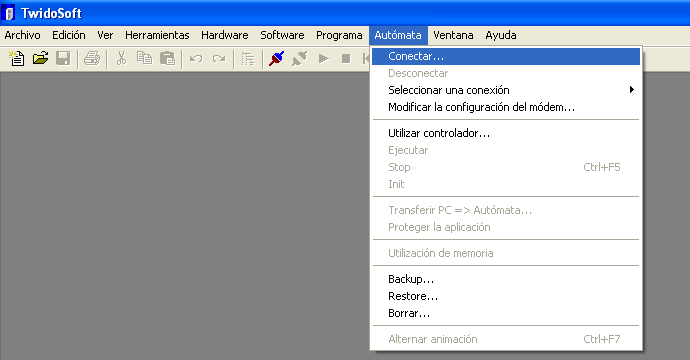
\includegraphics[width=0.4\textwidth]
	{Anexos/images/twidosoft.PNG}
    \end{center}\\
\hline
    Al conectarse y si existiese una diferencia entre las aplicaciones 
de la computadora y el \gls{plc} el software demandará elegir una opción.Cargar 
el programa desde la computadora al \gls{plc}
    &\begin{center}
      %\rule{0.4\textwidth}{0.3\textwidth}
      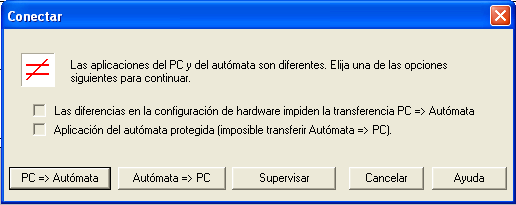
\includegraphics[width=0.4\textwidth]
	{Anexos/images/twidosoftcargar.PNG}
    \end{center}\\
\hline
    Poner a correr el programa, mediante el icono de Run.
    &\begin{center}
      %\rule{0.4\textwidth}{0.3\textwidth}
      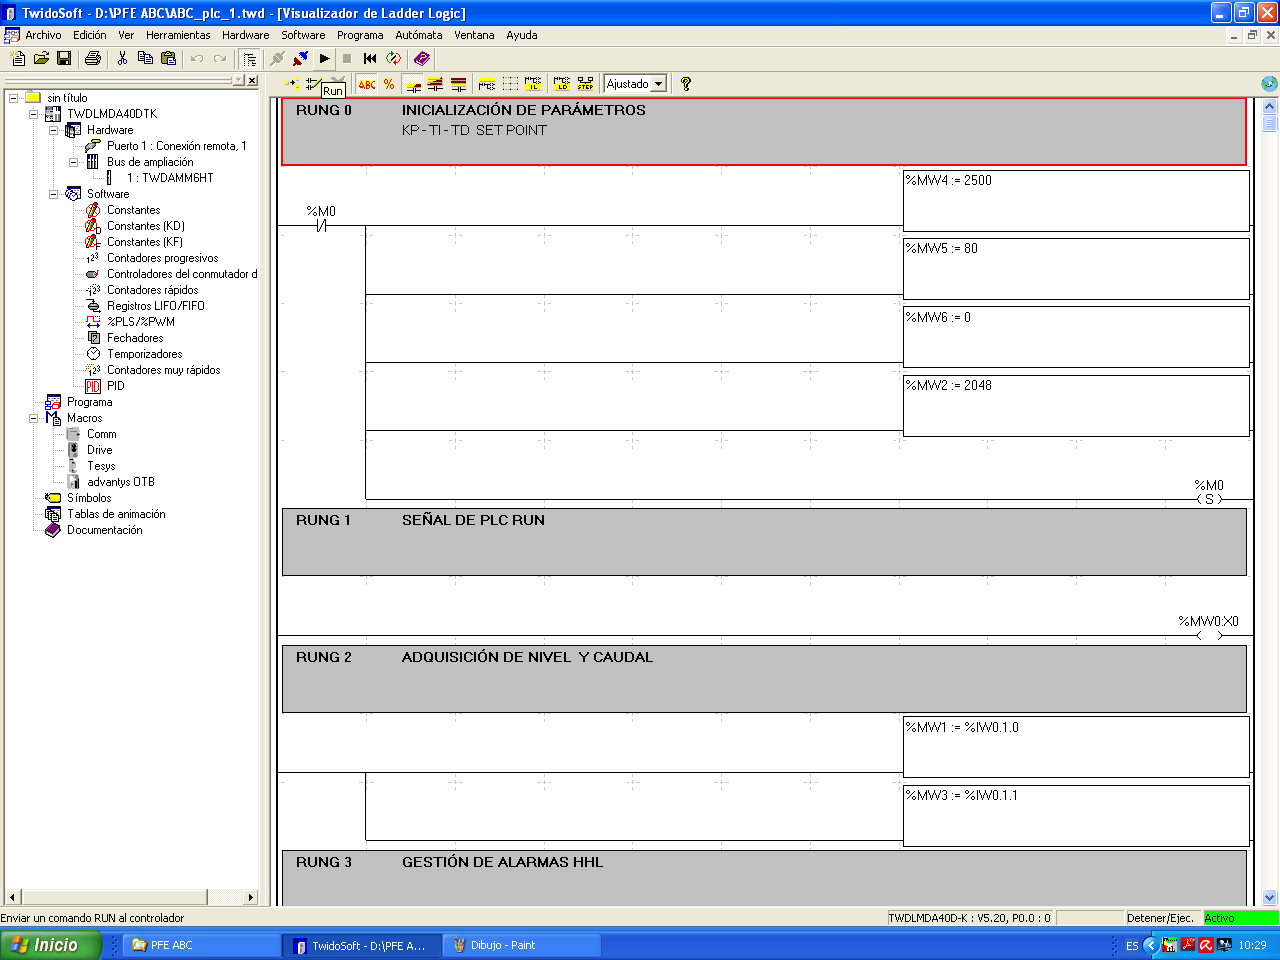
\includegraphics[width=0.4\textwidth]
	{Anexos/images/twidosoftrun.PNG}
    \end{center}\\
\hline
  Finalmente puede desconectarse del \gls{plc}
  &\begin{center}
    %\rule{0.4\textwidth}{0.3\textwidth}
    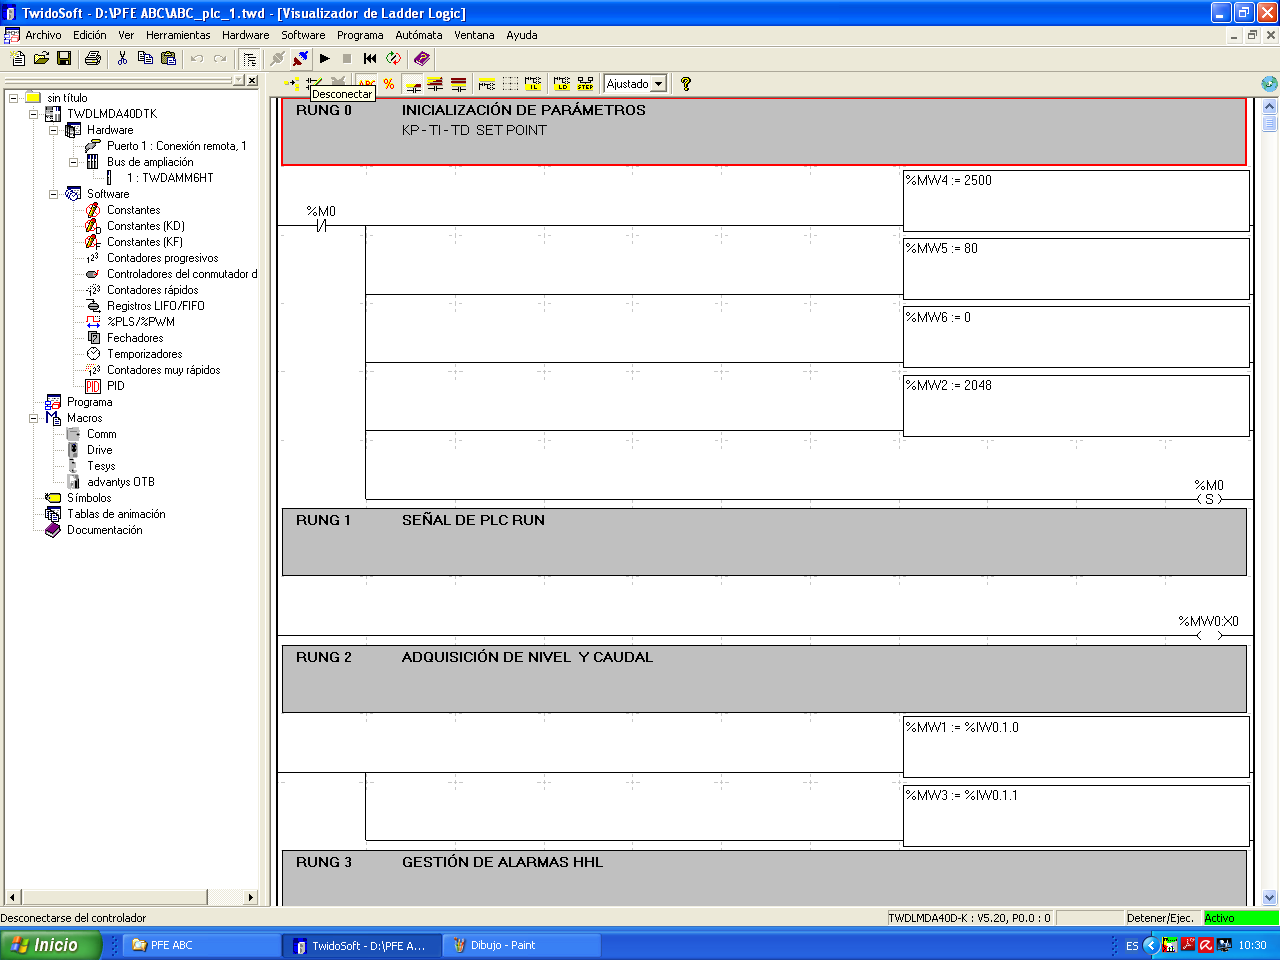
\includegraphics[width=0.4\textwidth]
      {Anexos/images/twidosoftdesc.PNG}
  \end{center}\\
\hline
\end{tabular}
\end{table}

% \begin{figure}[ht!]
% 	\centering
% 	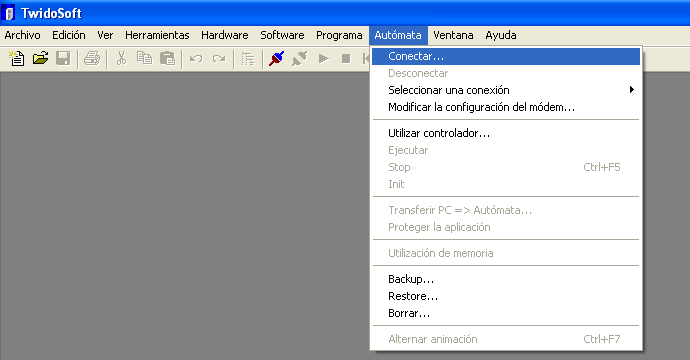
\includegraphics[scale=0.5]{Anexos/images/twidosoft.PNG}
% 	\caption{Esquema de la división del tiempo}
% 	\label{img:twidosoft}
% \end{figure}
% 
% \begin{figure}[ht!]
% 	\centering
% 	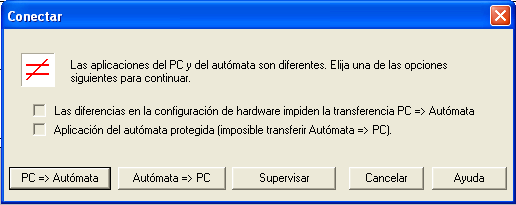
\includegraphics[scale=0.3]{Anexos/images/twidosoftcargar.PNG}
% 	\caption{Esquema de la división del tiempo}
% 	\label{img:twidosoftcargar}
% \end{figure}
% 
% \begin{figure}[ht!]
% 	\centering
% 	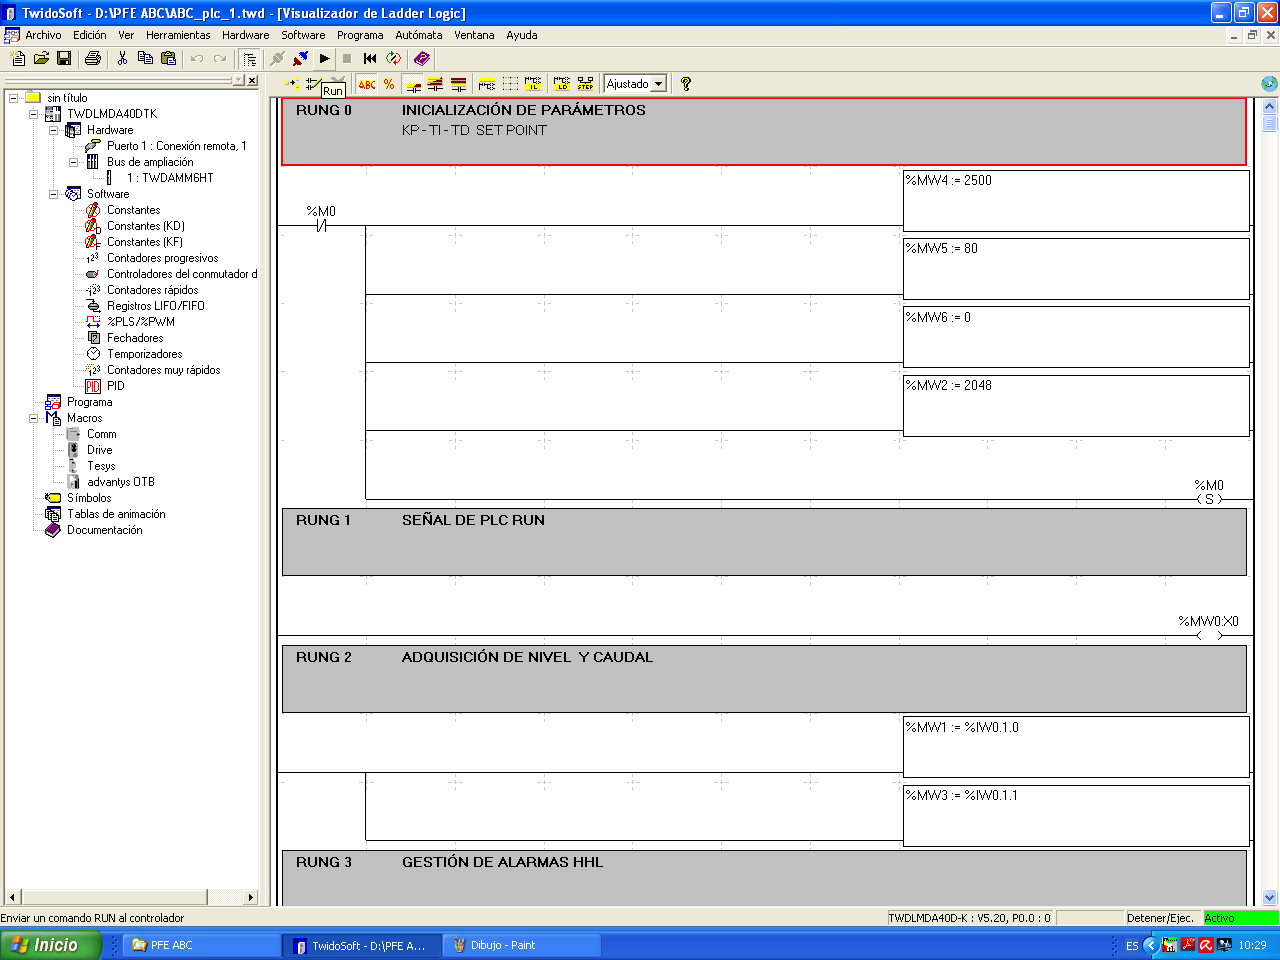
\includegraphics[scale=0.3]{Anexos/images/twidosoftrun.PNG}
% 	\caption{Esquema de la división del tiempo}
% 	\label{img:twidosoftrun}
% \end{figure}
% 
% \begin{figure}[ht!]
% 	\centering
% 	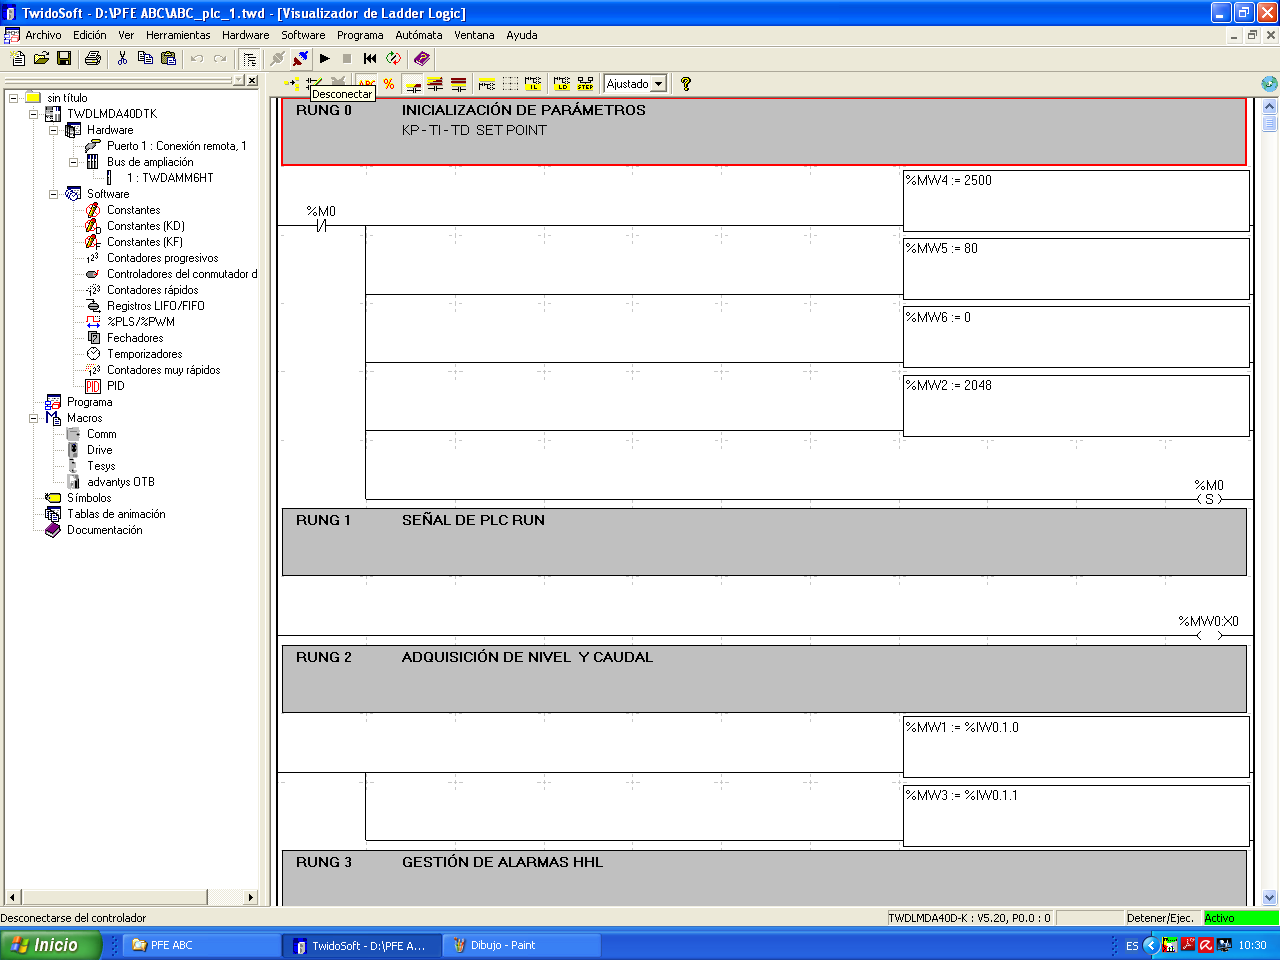
\includegraphics[scale=0.3]{Anexos/images/twidosoftdesc.PNG}
% 	\caption{Esquema de la división del tiempo}
% 	\label{img:twidosoftdesc}
% \end{figure}

\subsection{SCADA}
Normalmente, si el programa que corre en el \gls{plc} no ha sido cambiado, 
usted debería ser capaz de retomar la operación de la planta desde este punto. 
Para asegurarse de que el programa que corre en el \gls{plc} es el correcto 
refiérase a la sección \ref{anexo:operacionPLC} del Manual del Usuario.
\begin{lattention}
 Recuerde siempre realizar las verificaciones descriptas en la Sección 
\ref{anexo:verificaciones} del Manual del usuario antes de continuar con la 
operación de la planta.
\end{lattention}

\subsubsection{Iniciar P-CIM}
Para controlar el sistema desde el \gls{scada} de P-CIM de AFCON, es necesario 
iniciar P-CIM y verificar que el driver de Modbus se haya cargado correctamente:
\begin{table}[!ht]
\centering
\renewcommand*{\arraystretch}{0.01}
\begin{tabular}{*{2}{m{0.45\textwidth}}}
\hline
  Active P-CIM utilizando el Startup de P-CIM del grupo de aplicaciones de la 
carpeta AFCON P-CIM.
  &\begin{center}
    %\rule{0.4\textwidth}{0.3\textwidth}
    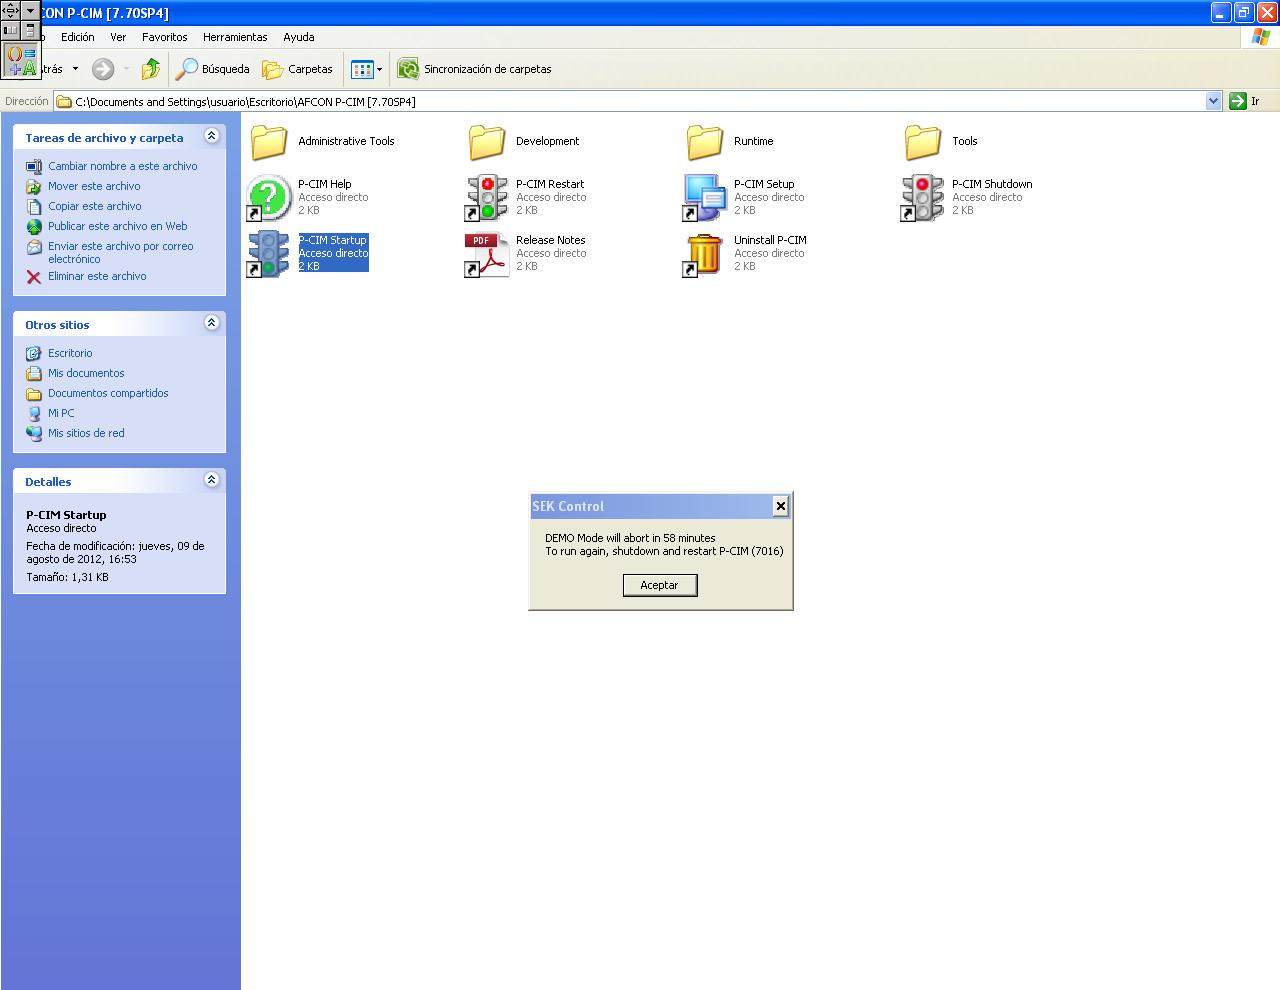
\includegraphics[width=0.4\textwidth]
      {Cap5-SCADA/images/startUp.jpeg}
  \end{center}\\
 \hline
   Verifique que en la ventana Alarm Summary aparezca el mensaje “MODBUS
  Driver successfully loaded” indicando que el driver halló la tabla de 
  comunicación y fue exitosamente cargado.
  &\begin{center}
    %\rule{0.4\textwidth}{0.3\textwidth}
    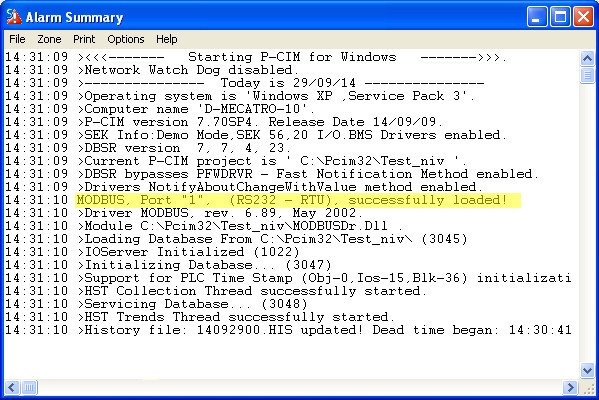
\includegraphics[width=0.4\textwidth]
      {Cap5-SCADA/images/alarm.jpeg}
  \end{center}\\
 \hline
\end{tabular}
\end{table}

\begin{lattention}
En el caso de que no se haya logrado cargar el driver Modbus refiérase a la 
Tab.\ref{tab:PropModbus} de la sección \ref{subsubsec:InforDriver}.
\end{lattention}

\subsubsection{Operators Workspace}
Para ejecutar el entorno gráfico del sistema \gls{scada} ejecute la aplicación 
Operator Workspace que se encuentra en el directorio \todo{agregar directorio}

A través de esta interfaz es posible manejar la planta. La misma se encuentra 
organizada en 4 bloques Principales.(Ver Fig.\todo{agregar foto})
\begin{enumerate}
 \item Control Automatico: En esta sección usted puede pasar al controlador de 
la planta la consigna/setpoint y las constantes del controlador Kp, Ti y Td.
 \item Control Manual: Este modo debe ser usado solamente como un medio para 
sacar a la planta de un estado de emergencia tras  haberse declarado una alarma 
por HHL o LLL.
 \item Sistema: En este apartado podemos ver el estado del actual del sistema. 
Es decir se muestran los valores de nivel y caudal actuales e históricos juntos 
con las alarmas.
 \item Activación: Desde estos controles se activa o se frena la planta.
\end{enumerate}

